\documentclass[10pt]{beamer}

%% Based on the original theme by Matthias Vogelgesang

\usetheme[progressbar=frametitle]{metropolis}
\usepackage{appendixnumberbeamer}
\usepackage{esvect}
\usepackage{amsmath}
\usepackage[utf8]{inputenc}
\usepackage[english]{babel}
\usepackage{minted}
\usepackage{xcolor}
\usepackage{multicol}



\usepackage{booktabs}
\usepackage{listings}
\usepackage[scale=2]{ccicons}

\usepackage{pgfplots}
\usepgfplotslibrary{dateplot}

\usepackage{xspace}
\newcommand{\themename}{\textbf{\textsc{metropolis}}\xspace}

%%%%%%%%%%%%%%%%%%%%%%%%%%%%
%% UNCC Theme Adjustments %%
%%%%%%%%%%%%%%%%%%%%%%%%%%%%
\definecolor{CanvasBG}{HTML}{FAFAFA}

% From the official style guide
\definecolor{UnccGreen}{HTML}{00703C}
\definecolor{UnccGold}{HTML}{B3A369}
\definecolor{UnccLightGreen}{HTML}{C3D7A4}
\definecolor{UnccYellow}{HTML}{F0CB00}
\definecolor{UnccOrange}{HTML}{F3901D}
\definecolor{UnccLightYellow}{HTML}{FFF6DC}
\definecolor{UnccBlue}{HTML}{00728F}
\definecolor{UnccPink}{HTML}{DE3A6E}
\definecolor{White}{HTML}{FFFFFF}
\definecolor{LightGray}{HTML}{DDDDDD}

% Supporting Color Palette
\definecolor{WarmGray}{HTML}{696158}
\definecolor{StoneGray}{HTML}{717C7D}
\definecolor{DarkGreen}{HTML}{2C5234}
\definecolor{LightGreen}{HTML}{509E2F}
\definecolor{BrightGold}{HTML}{F0CB00}

% Screamers
\definecolor{Royal}{HTML}{72246C}
\definecolor{Ocean}{HTML}{006BA6}
\definecolor{Flash}{HTML}{B52555}
\definecolor{Citrus}{HTML}{FFB81C}
\definecolor{Spring}{HTML}{CEDC00}

% Serenity
\definecolor{Garden}{HTML}{B7CE95}
\definecolor{Sand}{HTML}{F0E991}
\definecolor{Bloom}{HTML}{F1E6B2}
\definecolor{Clay}{HTML}{B7B09C}
\definecolor{Cloud}{HTML}{BAC5B9}

% Set colors here
\setbeamercolor{frametitle}{bg=UnccGreen}
\setbeamercolor{progress bar}{bg=BrightGold, fg=UnccGreen}
\setbeamercolor{alerted text}{fg=Flash}

\setbeamercolor{block title}{bg=LightGreen, fg=White}
\setbeamercolor{block title example}{bg=Ocean, fg=White}
\setbeamercolor{block title alerted}{bg=Citrus, fg=White}
\setbeamercolor{block body}{bg=CanvasBG}

\metroset{titleformat=smallcaps, progressbar=foot}

\makeatletter
\setlength{\metropolis@progressinheadfoot@linewidth}{2pt}
\setlength{\metropolis@titleseparator@linewidth}{2pt}
\setlength{\metropolis@progressonsectionpage@linewidth}{2pt}
%%%%%%%%%%%%%%%%%%%%%%%%%%%%
%% UNCC Theme Adjustments %%
%%%%%%%%%%%%%%%%%%%%%%%%%%%%

\newcommand{\RNum}[1]{\uppercase\expandafter{\romannumeral #1\relax}}


\title{Quake \RNum{3} Fast Inverse Square Root}
% \subtitle{A modern beamer theme for UNC Charlotte}
\date{\today}
% \date{}
\author{KHS Supriya}
% \institute{University of North Carolina at Charlotte}
% \titlegraphic{\hfill\includegraphics[height=1.5cm]{logo.pdf}}

\begin{document}

\maketitle

\begin{frame}{Table of contents}
  \setbeamertemplate{section in toc}[sections numbered]
  \tableofcontents%[hideallsubsections]
\end{frame}

\section[Games \& Inverse sqrt]{Introduction}

\begin{frame}[fragile]{Normalizing a Vector}
    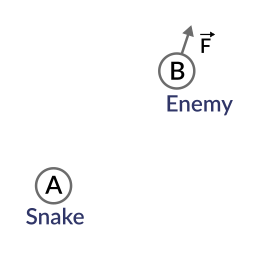
\includegraphics[width=4cm, height=4cm]{images/dot_product1.png}
    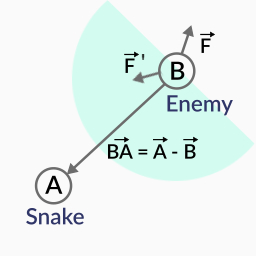
\includegraphics[width=4cm, height=4cm]{images/dot_product2_edited_twice.jpg}
    \newline
    \lstinputlisting[language=Python]{codes/snake_enemy.py}
\end{frame}


\begin{frame}[fragile]{Unit Vector}
    \begin{center}
        $\vec{u}^{\,} = \dfrac{x}{\sqrt{{x}^2+{y}^2+{z}^2}}\vec{i}^{\,} + \dfrac{y}{\sqrt{{x}^2+{y}^2+{z}^2}}\vec{j}^{\,} + \dfrac{z}{\sqrt{{x}^2+{y}^2+{z}^2}}\vec{k}^{\,}
        \newline
        \newline
        \newline
        \dfrac{1}{\sqrt{{x}^2+{y}^2+{z}^2}}
        $
    \end{center}
\end{frame}

% \section{The Default Approach}

\begin{frame}{So simple..?}
    \begin{center}
        \lstinputlisting[language=Python]{codes/naive.py}
    \end{center}
\end{frame}

\begin{frame}{Initial Estimate}
    \begin{center}
         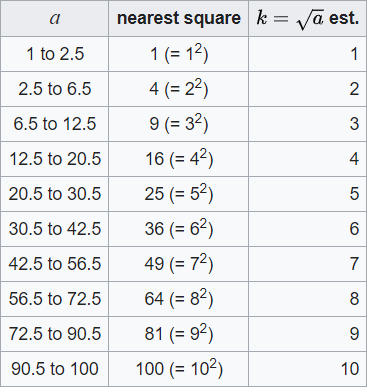
\includegraphics[scale=0.8]{images/look_up.PNG}
    \end{center}
\end{frame}

\begin{frame}{Newton's Method}
    % \begin{center}
        $x_{n+1} = x_n - \dfrac{f(x_n)}{f^\prime(x_n)}$
        \newline
        \newline
        $f(x) = {x}^2 - S \hspace{10mm}   f^\prime(x) = 2x$
        \newline
        \newline
        To find $\sqrt{2}$, Intial estimate $(x_1) = 1$
        \newline
        \newline
        $x_2 = \dfrac{1}{2}(x_1 + \dfrac{2}{x_1}) = \dfrac{17}{12}$
        \newline
        \newline
        $x_3 = \dfrac{1}{2}(x_2 + \dfrac{2}{x_2}) = \dfrac{577}{408}$
        \newline
        \newline
        ${x_3}^2 = \dfrac{332929}{166464} \approx 2.000006$
    % \end{center}
\end{frame}

% \subsection{Tricks}

\section{Fast Inverse Sqaure Root}

\begin{frame}{The Algorithm}
\lstinputlisting[basicstyle=\footnotesize, language=c]{codes/algorithm.c}
\end{frame}

\begin{frame}{IEE 754 - 1985}
    % \begin{center}
        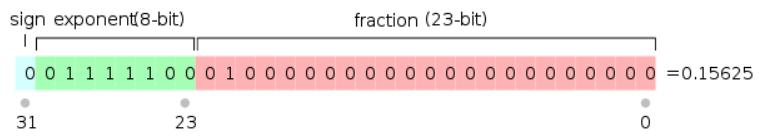
\includegraphics[scale=0.6]{images/IEEE_754.png}
        $
        0.15625_{10} = 0.00101_{2} \hspace{11mm} (\dfrac{1}{8} + \dfrac{1}{32})
        \newline
        \newline
        0.00101_{2} = 1.01_2 x {2}^{-3}
        \newline
        \newline
        sign = 0
        \newline
        \newline
        biased \hspace{1mm} exponent = -3 + "bias" = - 3 + 127 = 124
        \newline
        \newline
        fraction = .01000..._{2}
        $
    % \end{center}
\end{frame}

\begin{frame}{IEE 754 - 1985}
    % \begin{center}
        M \hspace{35mm} 01000000000000000000000
        \newline
        E \hspace{67mm} 01111100
        \newline
        \newline
        {\bf Bit Representation}
        \newline
        \newline
        {2}^{23}.E \hspace{18mm} 01111100 \hspace{1mm} 00000000000000000000000
        \newline
        \newline
        M + {2}^{23}.E \hspace{12mm} 01111100 \hspace{1mm} 01000000000000000000000
        \newline
        \newline
        {\bf Actual Number}
        \newline
        \newline
        $
        (1 + \dfrac{M}{{2}^{23}}) * {2}^{E - 127}
        $
    % \end{center}
\end{frame}


\begin{frame}{The trick}
    $
    k = log_2((1 + \dfrac{M}{{2}^{23}}) * {2}^{E - 127}) = log_2(1 + \dfrac{M}{{2}^{23}}) + E - 127
    \newline
    \newline
    $
    \begin{multicols}{2}
    $
        log(1+x) \approx x
        \newline
        \newline
        log(1+x) = x + \mu
        \newline
        \newline
       k = \dfrac{M}{{2}^{23}} + \mu + E - 127
       \newline
       \newline
       k = \dfrac{1}{{2}^{23}}(M + E * {2}^{23}) + \mu - 127
    $
    \columnbreak
    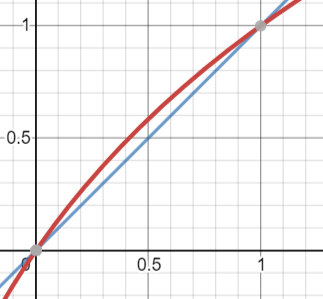
\includegraphics[scale=0.5]{images/log_graph.PNG}
    \end{multicols}
\end{frame}

\begin{frame}{The trick}
     $M + {2}^{23}.E$ \hspace{12mm} 01111100 \hspace{1mm} 01000000000000000000000
     \newline
     \newline
     \hspace{100}
     $ 
     \approx log(itself)
     $
\end{frame}

\begin{frame}{The Algorithm}
\lstinputlisting[basicstyle=\footnotesize, language=c]{codes/algorithm.c}
\end{frame}

\section{Evil Bit Hack}

\begin{frame}{Floating Point Trickery}
\begin{multicols}{2}
\lstinputlisting[basicstyle=\footnotesize, language=c]{codes/float_trick.c}
\columnbreak
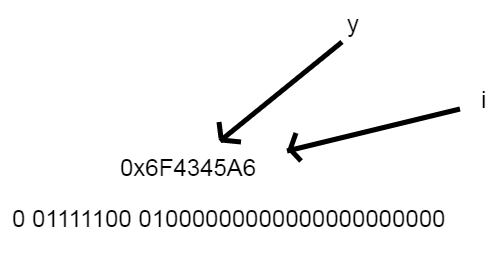
\includegraphics[scale=0.3]{images/pointers.png}
\end{multicols}
\end{frame}

\section{What the heck?}

\begin{frame}[fragile]{}
    \lstinputlisting[basicstyle=\footnotesize, language=c]{codes/heck.c}
    $ 
    log(\dfrac{1}{\sqrt{y}}) = -\dfrac{1}{2}log(y)
    \newline
    \newline
    log(y) = \dfrac{1}{{2}^{23}}(M + E * {2}^{23}) + \mu - 127
    \newline
    \newline
    log(y) = \dfrac{1}{{2}^{23}}(i) + \mu - 127 \approx i
    \newline
    \newline
    -\dfrac{1}{2}log(y) = - (i << 1)
    $
\end{frame}

\begin{frame}[fragile]{}
    $ 
    log(\gamma) = -\dfrac{1}{2}log(y)
    \newline
    \newline
    \dfrac{1}{{2}^{23}}(M_{\gamma} + E_{\gamma} * {2}^{23}) + \mu - 127 =
    -\dfrac{1}{2}(\dfrac{1}{{2}^{23}}(M_{y} + E_{y} * {2}^{23}) + \mu - 127)
    \newline
    \newline
    (M_{\gamma} + E_{\gamma} * {2}^{23}) = \dfrac{3}{2}{2}^{23}(127 - \mu) - \dfrac{1}{2}(M_y + {2}^{23}*E_y)
    \newline
    \newline
    (M_{\gamma} + E_{\gamma} * {2}^{23}) = 0x5f3759df - (i >> 1)
    
    $
\end{frame}

\begin{frame}{The Algorithm}
\lstinputlisting[basicstyle=\footnotesize, language=c]{codes/algorithm.c}
\end{frame}

\section{Newton Iteration}

\begin{frame}{Newton Iteration}
  \lstinputlisting[basicstyle=\footnotesize, language=c]{codes/newton.c}
  $
  f(y) = \dfrac{1}{{y}^2} - x
  \newline
  \newline
  y_{n + 1} = y_n - \dfrac{f(y_n)}{f^\prime(y_n)}
  \newline\newline
  y_{n + 1} = y_n(\dfrac{3}{2} - \dfrac{x}{2}{y_n}^2)
  $
\end{frame}

\begin{frame}{The Algorithm}
\lstinputlisting[basicstyle=\footnotesize, language=c]{codes/algorithm.c}
\end{frame}

{\setbeamercolor{palette primary}{fg=black, bg=yellow}
\begin{frame}[standout]
  Questions?
\end{frame}
}


\end{document}
